\section*{Problema 11.98, Z}
El extremo de un poste de altura $h$, descansa en una superficie horizontal áspera con $\mu _s = 0.3$. El extremo superior se sujeta con una cuerda fija a la superficie que forma un ángulo de $36.9 ^o$ con el poste. Se ejerce una fuerza horizontal $\vec{F}$ sobre el poste. $(a)$ Si $\vec{F}$ se aplica en el punto medio del poste, ¿qué valor máximo puede tener sin hacer que el poste resbale? $(b)$ Y si el punto de aplicación esta a $\frac{6}{10}$ de la longitud del poste desde la base? \textit{Reto: } Demuestre que si el punto de aplicación de la fuerza está a suficiente altura no puede hacerse que el poste resbale por más grande que sea la fuerza. Calcule esta altura crítica en términos de $h$ (altura del poste).


\begin{figure}[H]
	\centering
	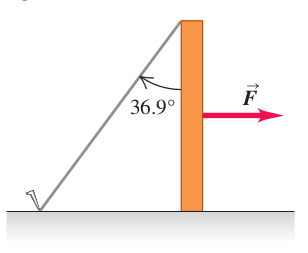
\includegraphics[scale=0.5]{./img/poste.png}
	\caption{Problema 11.98, Z.}
	\label{poste}
\end{figure}








%%%%